\maketitlesupplementary

% Sections are lettered; figures, tables, and equations continue the numbering of the submitted main paper
% (which ends at Figure 8, Table 3, and Eq. (11)).
\setcounter{figure}{8}\setcounter{table}{3}\setcounter{equation}{11}
\setcounter{section}{0}\renewcommand{\thesection}{\Alph{section}}
\raggedbottom  % columns end where the text ends; the kit's \flushbottom stretched short paragraphs apart
\renewcommand{\qedsymbol}{}  % no end-of-proof square; proofs end with a sentence

In this supplementary material, we provide the derivations and proofs omitted from the main paper (\cref{sec:supp-proofs}), implementation details (\cref{sec:supp-impl}), and additional results (\cref{sec:supp-results}).

\section{Derivations and Proofs}
\label{sec:supp-proofs}

For completeness, we first restate the allocation problem of the main paper. Let $\mathcal F$ and $\mathcal S$ be the candidate frames and subtitles, let $b_i\in[0,b_i^{\max}]$ be the token count of item $i\in\mathcal F\cup\mathcal S$, and let $v_i(b_i)=b_i/(b_i+\tau_i)$ be its token value, where $\tau_i$ is $\tau_{\text{frame}}$ for a frame and $\tau_{\text{text}}$ for a subtitle. \name solves
\begin{equation}
\begin{aligned}
  \max_{\mathbf b}\quad & \sum_{i\in\mathcal F} r_i(q,\mathbf b)\,v_i(b_i)+\beta\sum_{i\in\mathcal S} r_i(q,\mathbf b)\,v_i(b_i)\\
  \text{s.t.}\quad & \sum_{i\in\mathcal F\cup\mathcal S} b_i\le B ,
\end{aligned}
\label{eq:supp-allocation}
\end{equation}
where the allocation-dependent relevance $r_i(q,\mathbf b)$ discounts the retrieval relevance $r_i(q)$ of item $i$ by the token values of the similar items of its modality $\mathcal M_i\in\{\mathcal F,\mathcal S\}$:
\begin{equation}
  r_i(q,\mathbf b)=r_i(q)-\eta\sum_{j\in\mathcal M_i}s_{ij}\,v_j(b_j) .
\label{eq:supp-cond}
\end{equation}
Here, $s_{ij}$ is the cosine similarity between the embeddings of items $i$ and $j$, and $\eta\ge0$ is the redundancy penalty.

\subsection{NP-Hardness of the Discrete Problem}
\label{sec:supp-nphard}

The VLM consumes whole tokens, so the allocation problem of \cref{eq:supp-allocation} is originally discrete: every token count $b_i$ is an integer in $\{0,1,\dots,b_i^{\max}\}$. We show that this discrete problem is NP-hard, so that no polynomial-time algorithm solves it exactly unless $\mathrm{P}=\mathrm{NP}$. The hardness holds even when every item has a single token, in which case allocation reduces to selection. As in \cref{eq:supp-allocation}, an instance specifies the embeddings only through their similarities $s_{ij}$.

\smallskip
\noindent\textbf{Proposition 2.} \textit{Maximizing \cref{eq:supp-allocation} over integer token counts $b_i\in\{0,1,\dots,b_i^{\max}\}$ is NP-hard.}

\begin{proof}
We reduce from the independent set problem, which is NP-complete~\cite{karp1972,garey1979}: given a graph $G=(V,E)$ with $n$ vertices and an integer $k$, decide whether $G$ contains $k$ vertices of which no two are adjacent.

Given $G$ and $k$, we construct an instance with one frame per vertex and no subtitles. Every frame has $b_i^{\max}=1$, $\tau_i=1$, and retrieval relevance $r_i(q)=1/n$, and we set $\eta=1/n$ and $B=k$. The similarities are $s_{ii}=1$, $s_{ij}=1/n$ if $\{i,j\}\in E$, and $s_{ij}=0$ otherwise, i.e., $\mathbf S=\mathbf I+\mathbf A/n$, where $\mathbf A$ is the adjacency matrix of $G$. Every eigenvalue of $\mathbf A$ has magnitude at most the maximum degree, which is at most $n-1$, so every eigenvalue of $\mathbf S$ is positive. $\mathbf S$ is, therefore, positive definite with unit diagonal, i.e., the Gram matrix of $n$ unit vectors, whose cosine similarities are exactly $s_{ij}$. The construction takes polynomial time.

In this instance, each frame receives either no token, with token value $0$, or one token, with token value $v_i(1)=1/2$. Let $X$ be the set of frames that receive a token, and let $e(X)$ be the number of edges of $G$ with both endpoints in $X$. The budget requires $|X|\le k$, and the objective of \cref{eq:supp-allocation} becomes
\begin{equation}
\begin{aligned}
  J(X)&=\frac{|X|}{2n}-\frac{1}{4n}\sum_{i,j\in X}s_{ij}
       =\frac{|X|}{2n}-\frac{|X|}{4n}-\frac{e(X)}{2n^2}\\
      &=\frac{|X|}{4n}-\frac{e(X)}{2n^2} .
\end{aligned}
\label{eq:supp-nphard}
\end{equation}
Since $e(X)\ge0$ and $|X|\le k$, every feasible allocation satisfies $J(X)\le k/(4n)$, with equality if and only if $|X|=k$ and $e(X)=0$, i.e., if and only if $X$ is an independent set of size $k$. Hence, $G$ contains an independent set of size $k$ if and only if the optimal value of the discrete problem is $k/(4n)$. A polynomial-time algorithm for the discrete problem would thus decide the independent set problem in polynomial time, which completes the proof.
\end{proof}

\noindent The construction relies on the redundancy penalty, which couples the items: without it ($\eta=0$), giving one token to any $k$ frames is optimal. In the continuous relaxation, the same coupling still yields a convex program, because $\mathbf S$ is positive semidefinite (\cref{sec:supp-convex}). \name, therefore, solves the relaxation and rounds its solution down to whole tokens.

\subsection{Convexity of the Continuous Relaxation}
\label{sec:supp-convex}

The continuous relaxation lets each token count $b_i$ take any real value in $[0,b_i^{\max}]$. We show that, after a change of variables, this relaxation maximizes a concave function over a convex set. Every later result relies on this property.

We change variables from the token counts to the token values $z_i=v_i(b_i)$, and write $\mathbf b$ and $\mathbf z$ for the vectors over all items. Since $v_i$ is strictly increasing, this change of variables is invertible, with
\begin{equation}
  b_i=v_i^{-1}(z_i)=\frac{\tau_i z_i}{1-z_i} ,
\label{eq:supp-inverse}
\end{equation}
where $0\le z_i\le z_i^{\max}=v_i(b_i^{\max})<1$.
The budget $B$ therefore restricts the token values to the feasible set
\begin{equation}
  \mathcal Z=\Big\{\mathbf z:\ 0\le z_i\le z_i^{\max},\ \ \sum_{i}\frac{\tau_i z_i}{1-z_i}\le B\Big\} .
\label{eq:supp-feasible}
\end{equation}
Each function $\tau_i z_i/(1-z_i)$ is convex on $[0,1)$, because its second derivative $2\tau_i/(1-z_i)^3$ is positive. The budget constraint thus keeps a convex function below $B$, so $\mathcal Z$ is convex, and it is compact because it is closed and bounded.

The objective, in turn, is concave in the token values. Substituting \cref{eq:supp-cond} into \cref{eq:supp-allocation} gives
\begin{equation}
  J(\mathbf z)=\bar{\mathbf r}^{\top}\mathbf z-\eta\,\mathbf z^{\top}\mathbf S\mathbf z ,
\label{eq:supp-quadratic}
\end{equation}
where $\bar r_i=r_i(q)$ for a frame and $\bar r_i=\beta\,r_i(q)$ for a subtitle, and the similarity matrix $\mathbf S$ is block-diagonal, with the frame similarity matrix and the $\beta$-scaled subtitle similarity matrix as its blocks. Each block contains the cosine similarities between the embeddings of one modality, including the diagonal entries $s_{ii}=1$. The frame block is, therefore, a Gram matrix of normalized embeddings and the subtitle block is a positive multiple of one, so $\mathbf S$ is positive semidefinite. Since $\eta\ge0$, $J$ is concave. Maximizing $J$ over $\mathcal Z$ is thus a convex program, in which every local maximum is a global maximum~\cite{boyd2004}.

\subsection{Derivation of Water-Filling}
\label{sec:supp-waterfill}

We now derive the water-filling allocation of the main paper as the unique solution of the subproblem in which the relevance of each item is fixed to $\bar r_i>0$:
\begin{equation}
\begin{aligned}
  \max_{\mathbf b}\quad & \sum_i \bar r_i\,\frac{b_i}{b_i+\tau_i}\\
  \text{s.t.}\quad & \sum_i b_i\le B,\quad 0\le b_i\le b_i^{\max} .
\end{aligned}
\label{eq:supp-fixed}
\end{equation}
We solve this subproblem through its Lagrangian dual. The idea is to replace the budget by a price per token, let each item acquire tokens at that price, and then adjust the price until the budget is spent. We introduce a multiplier $\lambda\ge0$ for the budget constraint and keep the bounds $0\le b_i\le b_i^{\max}$ as the domain of $\mathbf b$, which gives the Lagrangian
\begin{equation}
  \mathcal L(\mathbf b,\lambda)=\sum_i \bar r_i\,\frac{b_i}{b_i+\tau_i}-\lambda\Big(\sum_i b_i-B\Big) .
\label{eq:supp-lagrangian}
\end{equation}
The subproblem is equivalent to $\max_{\mathbf b}\min_{\lambda\ge0}\mathcal L(\mathbf b,\lambda)$, and its dual is $\min_{\lambda\ge0}\max_{\mathbf b}\mathcal L(\mathbf b,\lambda)$. Strong duality holds because the objective is concave, the constraints are linear, and $\mathbf b=\mathbf 0$ is strictly feasible~\cite{boyd2004}. Hence, the two problems attain the same value, and the solution of the subproblem maximizes $\mathcal L(\cdot,\lambda^\star)$ at the dual optimum $\lambda^\star$.

\paragraph{Inner maximization.}
For a fixed $\lambda>0$, the Lagrangian separates over the items, and each item solves
\begin{equation}
  \max_{0\le b_i\le b_i^{\max}}\ \bar r_i\,\frac{b_i}{b_i+\tau_i}-\lambda\,b_i .
\label{eq:supp-item}
\end{equation}
This objective is strictly concave. Setting its derivative to zero gives
\begin{equation}
  \frac{\bar r_i\,\tau_i}{(b_i+\tau_i)^2}=\lambda ,
\label{eq:supp-stationarity}
\end{equation}
and clipping the solution to the domain gives the unique maximizer
\begin{equation}
  b_i(\lambda)=\left[\sqrt{\bar r_i\tau_i/\lambda}-\tau_i\right]_0^{b_i^{\max}} ,
\label{eq:supp-waterfill}
\end{equation}
which is the water-filling allocation of the main paper. Intuitively, each item acquires tokens until its marginal gain falls to the price $\lambda$. An item thus receives no tokens when its marginal gain at zero tokens, $\bar r_i/\tau_i$, does not exceed $\lambda$, and it receives its full token count when its marginal gain at $b_i^{\max}$ is at least $\lambda$. In iterative water-filling, the discounted relevance of an item can be non-positive. Such an item cannot increase the objective and receives no tokens.

\paragraph{Outer minimization.}
Substituting \cref{eq:supp-waterfill} into \cref{eq:supp-lagrangian} gives the dual function $g(\lambda)=\mathcal L(\mathbf b(\lambda),\lambda)$, which is convex in the single variable $\lambda$ with derivative
\begin{equation}
  g'(\lambda)=B-\sum_i b_i(\lambda) .
\label{eq:supp-dual}
\end{equation}
If $\sum_i b_i^{\max}\le B$, the budget is not binding and every item receives its full token count. Otherwise, the dual optimum $\lambda^\star$ satisfies $g'(\lambda^\star)=0$, i.e., the allocation spends exactly the budget. Because of the clipping, this equation has no closed-form solution in general. However, each $b_i(\lambda)$ is continuous and non-increasing in $\lambda$, and all of them vanish once $\lambda\ge\max_i\bar r_i/\tau_i$. A bisection over $\lambda\in(0,\max_i\bar r_i/\tau_i]$ therefore finds $\lambda^\star$. Since the inner maximizer is unique, the resulting allocation $\mathbf b(\lambda^\star)$ is the unique solution of \cref{eq:supp-fixed}.

\subsection{Proof of Proposition 1}
\label{sec:supp-convergence}

\noindent\textbf{Proposition 1} (restated)\textbf{.} \textit{Let $J^\star$ be the global maximum of \cref{eq:supp-allocation} over continuous token allocations, and let $J^{(\ell)}$ be the objective value after $\ell$ iterations of Algorithm~1 of the main paper. Then}
\begin{equation}
  J^\star-J^{(\ell)}\le\frac{4\,\eta\,\sigma_{\max}D^2}{\ell+2}=O\Big(\frac{1}{\ell}\Big) ,
\label{eq:supp-rate}
\end{equation}
\textit{where $\sigma_{\max}$ is the largest eigenvalue of the frame and $\beta$-scaled subtitle similarity matrices and $D$ is the diameter of the feasible token-value set under budget $B$.}

\smallskip
The proof follows the standard analysis of the Frank--Wolfe method~\cite{jaggi2013}, applied to the token values of \cref{sec:supp-convex}. It uses the gradient $\nabla J(\mathbf z)=\bar{\mathbf r}-2\eta\,\mathbf S\mathbf z$, which is the discounted relevance $\tilde{\mathbf r}$ of Eq.~(6) of the main paper, and the constant $C=2\eta\,\sigma_{\max}$, which bounds the curvature of $J$. The diameter $D$ is the largest distance between two points of $\mathcal Z$. The proof rests on two lemmas. The first bounds how far the current token values are from the optimum, and the second bounds how much one iteration improves the objective.

\begin{lemma}[Distance to the optimum]
\label{lem:gap}
For every $\mathbf z\in\mathcal Z$,
\begin{equation}
  J^\star-J(\mathbf z)\le\max_{\mathbf y\in\mathcal Z}\,\nabla J(\mathbf z)^{\top}(\mathbf y-\mathbf z) .
\label{eq:supp-lem-gap}
\end{equation}
\end{lemma}
\begin{proof}
Let $\mathbf z^{\rm opt}$ be a maximizer of $J$ over $\mathcal Z$. Since $J$ is concave, its linear approximation at $\mathbf z$ lies above it, so $J^\star=J(\mathbf z^{\rm opt})\le J(\mathbf z)+\nabla J(\mathbf z)^{\top}(\mathbf z^{\rm opt}-\mathbf z)$. The right-hand side is at most the maximum over all $\mathbf y\in\mathcal Z$.
\end{proof}

\noindent Intuitively, the best improvement that the linear approximation predicts is never smaller than the remaining gap. One water-filling pass solves exactly this maximization. In token values, the objective of \cref{eq:supp-fixed} with relevances $\nabla J(\mathbf z)$ is the linear function $\nabla J(\mathbf z)^{\top}\mathbf y$, and its constraints define $\mathcal Z$.

\begin{lemma}[Progress of one step]
\label{lem:step}
For every $\mathbf z,\mathbf s\in\mathcal Z$ and $\gamma\in[0,1]$,
\begin{equation}
\begin{aligned}
  J\big(\mathbf z+\gamma(\mathbf s-\mathbf z)\big)\ge{}& J(\mathbf z)+\gamma\,\nabla J(\mathbf z)^{\top}(\mathbf s-\mathbf z)\\
  &-\frac{C}{2}\gamma^2D^2 .
\end{aligned}
\label{eq:supp-lem-step}
\end{equation}
\end{lemma}
\begin{proof}
Write $\mathbf d=\gamma(\mathbf s-\mathbf z)$. Since $J$ is quadratic, its second-order expansion is exact: $J(\mathbf z+\mathbf d)=J(\mathbf z)+\nabla J(\mathbf z)^{\top}\mathbf d-\eta\,\mathbf d^{\top}\mathbf S\mathbf d$. The last term is at least $-\eta\,\sigma_{\max}\|\mathbf d\|^2=-\frac{C}{2}\|\mathbf d\|^2$, and $\|\mathbf d\|\le\gamma D$.
\end{proof}

\noindent That is, a step of size $\gamma$ toward $\mathbf s$ gains at least a fraction $\gamma$ of the improvement predicted for a full step, minus a curvature term that shrinks with $\gamma^2$.

\begin{proof}[Proof of Proposition 1]
We first derive a recursion for the remaining gap and then solve it by induction. Let $\mathbf z^{(\ell-1)}$ be the token values before iteration $\ell$, with $\mathbf z^{(0)}=\mathbf 0$, and let $h_\ell=J^\star-J(\mathbf z^{(\ell)})$ be the remaining gap. Iteration $\ell$ runs water-filling with the discounted relevance $\nabla J(\mathbf z^{(\ell-1)})$, which returns the maximizer $\mathbf s$ of the right-hand side of \cref{eq:supp-lem-gap} ($\mathbf z^\star$ in the main paper), and moves to $\mathbf z^{(\ell)}=\mathbf z^{(\ell-1)}+\gamma_\ell(\mathbf s-\mathbf z^{(\ell-1)})$ with $\gamma_\ell=2/(\ell+1)$. This point lies in $\mathcal Z$ because $\mathcal Z$ is convex.

Applying \cref{lem:step} with $\mathbf z=\mathbf z^{(\ell-1)}$ and $\gamma=\gamma_\ell$ gives
\begin{align*}
  J(\mathbf z^{(\ell)})
  &\ge J(\mathbf z^{(\ell-1)})+\gamma_\ell\,\nabla J(\mathbf z^{(\ell-1)})^{\top}(\mathbf s-\mathbf z^{(\ell-1)})\\
  &\qquad-\frac{C}{2}\gamma_\ell^2D^2\\
  &\ge J(\mathbf z^{(\ell-1)})+\gamma_\ell\,h_{\ell-1}-\frac{C}{2}\gamma_\ell^2D^2 ,
\end{align*}
where the second inequality uses \cref{lem:gap}. Subtracting both sides from $J^\star$ gives
\begin{equation}
  h_\ell\le(1-\gamma_\ell)\,h_{\ell-1}+\frac{C}{2}\gamma_\ell^2D^2 .
\label{eq:supp-recursion}
\end{equation}
Each iteration thus removes a fraction $\gamma_\ell$ of the remaining gap and adds a curvature term of order $\gamma_\ell^2$.

We now show $h_\ell\le2CD^2/(\ell+2)$ by induction. For $\ell=1$, the step size is $\gamma_1=1$, and \cref{eq:supp-recursion} gives $h_1\le CD^2/2\le2CD^2/3$. For $\ell\ge2$, assume the claim for $\ell-1$, i.e., $h_{\ell-1}\le2CD^2/(\ell+1)$. Then
\begin{align*}
  h_\ell&\overset{\text{(a)}}{\le}\frac{\ell-1}{\ell+1}\,h_{\ell-1}+\frac{2CD^2}{(\ell+1)^2}\\
  &\overset{\text{(b)}}{\le}\frac{\ell-1}{\ell+1}\cdot\frac{2CD^2}{\ell+1}+\frac{2CD^2}{(\ell+1)^2}\\
  &=\frac{2CD^2\,\ell}{(\ell+1)^2}\overset{\text{(c)}}{\le}\frac{2CD^2}{\ell+2} ,
\end{align*}
where (a) substitutes $\gamma_\ell=2/(\ell+1)$ into \cref{eq:supp-recursion}, (b) applies the induction hypothesis, and (c) uses $\ell(\ell+2)\le(\ell+1)^2$. Substituting $C=2\eta\,\sigma_{\max}$ gives \cref{eq:supp-rate}, which completes the proof.
\end{proof}

\noindent Proposition~1 yields two implications. First, without the redundancy penalty ($\eta=0$), the bound is zero, so the first iteration, which is plain water-filling, is already optimal. Second, since every token value lies in $[0,1)$, the diameter satisfies $D^2\le|\mathcal F|+|\mathcal S|$, so the numerator of the bound is at most $4\,\eta\,\sigma_{\max}(|\mathcal F|+|\mathcal S|)$. The bound holds for the continuous allocation, which \name rounds down to whole tokens afterward.

\subsection{Suboptimality of Prior Allocation Rules}
\label{sec:supp-prior}

The main paper states that neither proportional allocation~\cite{luo2025quota} nor tiered allocation~\cite{zhang2025qframe} maximizes the fixed-relevance objective of \cref{eq:supp-fixed}. This section proves both statements.

\begin{lemma}[Proportional allocation]
\label{lem:proportional}
Suppose at least three items have pairwise distinct relevances $\bar r_i>0$ and share the same parameter $\tau$, and let $b_i=c\,\bar r_i$ with $c>0$ satisfy $0<b_i<b_i^{\max}$ for these items. Then this allocation does not maximize \cref{eq:supp-fixed}.
\end{lemma}
\begin{proof}
By \cref{sec:supp-waterfill}, an optimal allocation requires all items with $0<b_i<b_i^{\max}$ to share the same marginal gain, i.e., $\bar r_i\tau/(c\,\bar r_i+\tau)^2=\lambda$ for some $\lambda>0$. Rearranging this equation shows that every such relevance is a root of the quadratic $\lambda c^2x^2+(2\lambda c\tau-\tau)x+\lambda\tau^2=0$ in $x$. A quadratic has at most two distinct roots, which contradicts the three pairwise distinct relevances.
\end{proof}

\noindent Intuitively, proportional allocation would equalize the marginal gains only if the token value grew like $\log b_i$, which never saturates. With a saturating token value, proportional allocation keeps adding tokens to the most relevant items after their token value has saturated, and takes these tokens from less relevant items that would still benefit.

\begin{lemma}[Tiered allocation]
\label{lem:tiered}
Suppose two items of the same tier have distinct relevances $\bar r_i\ne\bar r_j$, share the same parameter $\tau$, and receive the same token count $b$ with $0<b<\min(b_i^{\max},b_j^{\max})$. Then this allocation does not maximize \cref{eq:supp-fixed}.
\end{lemma}
\begin{proof}
An optimal allocation requires equal marginal gains for the two items, $\bar r_i\tau/(b+\tau)^2=\bar r_j\tau/(b+\tau)^2$, which holds only if $\bar r_i=\bar r_j$.
\end{proof}

\noindent Intuitively, the more relevant of the two items still gains more from its next token, so moving one token to it raises the objective.

In both cases, the water-filling allocation of \cref{eq:supp-waterfill} is the unique maximizer and, therefore, attains a strictly higher objective within the same budget.

\section{Implementation Details}
\label{sec:supp-impl}

\subsection{Settings of \name}
\label{sec:supp-settings}

\Cref{tab:supp-hparams} lists the settings of \name, which are the same for Qwen3-VL-8B~\cite{bai2025qwen3vl} and InternVL3.5-4B~\cite{wang2025internvl35}. SigLIP~2 embeds the query and the candidate frames, and BGE embeds the query and the candidate subtitles. Within each modality, we standardize the cosine similarities between the query and the candidate items to zero mean and unit variance and turn them into the retrieval relevance $r_i(q)$ with a softmax of temperature $T$. The token value parameters $\tau_{\text{frame}}$ and $\tau_{\text{text}}$ set how quickly the token value of an item saturates and are fitted offline by least squares to the validation measurements of Sec.~3.2 of the main paper. The subtitle weight $\beta$ scales the relevance of subtitles relative to that of frames, and the redundancy penalty $\eta$ scales the discount that an item receives from similar items. Iterative water-filling runs for $L$ iterations and finds $\lambda$ in each iteration by bisection. In multi-turn conversations, the attention weight $\omega$ controls the contribution of attention to the relevance of cached items. The token budget $B$ sets the compute of each experiment, which we report in TFLOPs with each result.

\begin{table}[!htb]
  \centering
  \footnotesize
  \renewcommand{\arraystretch}{1.15}
  \setlength{\tabcolsep}{4pt}
  \begin{tabular}{l l}
    \toprule
    Setting & Value \\
    \midrule
    Frame relevance encoder & SigLIP 2 (so400m-patch14-384)~\cite{siglip2} \\
    Subtitle relevance encoder & BGE (base-en-v1.5)~\cite{bge} \\
    Relevance temperature $T$ & 0.63 \\
    \addlinespace[3pt]
    Token value parameter $\tau_{\text{frame}}$ & 38 \\
    Token value parameter $\tau_{\text{text}}$ & 13.6 \\
    Subtitle weight $\beta$ & 0.5 \\
    Redundancy penalty $\eta$ & $2.67\times10^{-5}$ \\
    \addlinespace[3pt]
    Iterations $L$ & 20 \\
    Bisection steps per iteration & 60 \\
    \addlinespace[3pt]
    Attention weight $\omega$ (multi-turn) & 0.5 \\
    \bottomrule
  \end{tabular}
  \caption{Settings of \name, shared by both VLMs.}
  \label{tab:supp-hparams}
\end{table}

\subsection{Answer Prompt}
\label{sec:supp-prompt}

All methods answer the multiple-choice questions with the prompt in \cref{fig:supp-prompt}. Each frame is preceded by its timestamp, and on Video-MME the selected subtitles precede the question. The prediction is the option letter to which the VLM assigns the highest probability.

\begin{figure}[!htb]
\begin{tcolorbox}[colframe=gray, colback=white, colbacktitle=gray!10, coltitle=black,
    boxrule=0.4mm, arc=1mm, left=4pt, right=4pt, top=3pt, bottom=3pt,
    fonttitle=\bfseries\small, title={Prompt: Multiple-choice answering}]
\small
\textcolor{gray}{\textit{$\langle$4.0 seconds$\rangle$ [frame] \ $\langle$12.0 seconds$\rangle$ [frame] \ \dots}}

\smallskip
Subtitles of the video: \textcolor{gray}{\textit{[subtitles]}}

\smallskip
Select the best answer to the following multiple-choice question based on the video. Respond with only the letter of the correct option.

\smallskip
Question: \textcolor{gray}{\textit{[question]}}\\
Options:\\
A. \textcolor{gray}{\textit{[option]}}\\
B. \textcolor{gray}{\textit{[option]}}\\
\textcolor{gray}{\dots}

\smallskip
The best answer is:
\end{tcolorbox}
\vspace{-2mm}
\caption{Answer prompt shared by all methods. Gray italic text marks the inputs of each question.}
\label{fig:supp-prompt}
\end{figure}

\subsection{Baseline Implementations}
\label{sec:supp-baselines}

We compare all methods under the same conditions, so that differences in accuracy come from which evidence each method selects and how it divides the token budget. All methods select from the same candidate frames and answer with the same VLM and prompt (\cref{sec:supp-prompt}) within the same token budget. On Video-MME, every baseline also receives the subtitles aligned with the frames it selects, counted within that budget. Every method that scores query--frame relevance with an image--text encoder uses the same SigLIP~2 similarities as \name, so that no method gains from a stronger encoder. QuoTA keeps its own scorer, a VLM judge that is part of the method itself. For methods that call a VLM more than once, every call counts toward their compute. Each baseline otherwise keeps the settings recommended by its authors and is implemented as follows.

\begin{itemize}\setlength{\itemsep}{0pt}\setlength{\parskip}{0pt}\setlength{\topsep}{2pt}
  \item \textbf{Uniform sampling}: evenly spaced frames, each with the same token count.
  \item \textbf{Top-K}: as described in the main paper.
  \item \textbf{FOCUS}~\cite{zhu2026focus}: released code, with SigLIP~2 similarities in place of its BLIP scores.
  \item \textbf{Q-Frame}~\cite{zhang2025qframe}: released code, with SigLIP~2 similarities in place of its Long-CLIP scores and its three resolution tiers scaled to fill the token budget.
  \item \textbf{QuoTA}~\cite{luo2025quota}: released code, with its default prompts and its Qwen2-VL-2B judge.
  \item \textbf{AdaAlloc}~\cite{an2026adaalloc}: re-implemented from its paper, with SigLIP~2 similarities in place of its PE-Core scores. Since it makes three VLM calls per question, we scale the token budget of each call so that its total compute matches that of the other methods.
\end{itemize}

% Declared at the end of B.3 so that Table 5 is placed at the top of the column that holds C.2.
\begin{table}[t]
  \centering
  \footnotesize
  \setlength{\tabcolsep}{3.4pt}
  \renewcommand{\arraystretch}{1.15}
  \begin{tabular}{r r r r r r}
    \toprule
    \multirow{2}{*}{Frames} & \multicolumn{4}{c}{Solving time (s)} & \multirow{2}{*}{Speedup} \\
    \cmidrule(lr){2-5}
    & Gurobi~\cite{gurobi} & SCIP~\cite{scip} & CVXPY~\cite{cvxpy} & Ours & \\
    \midrule
    30    & 0.04 & 1.9   & 0.010 & 0.006 & 1.8--349$\times$ \\
    60    & 0.03 & 4.0   & 0.013 & 0.007 & 1.8--539$\times$ \\
    120   & 0.09 & 9.7   & 0.039 & 0.009 & 4.3--1,061$\times$ \\
    240   & 0.20 & 23.9  & 0.040 & 0.031 & 1.3--771$\times$ \\
    420   & 0.56 & 51.7  & 0.080 & 0.025 & 3.2--2,060$\times$ \\
    1,800 & 3.01 & 600+ & 0.76 & 0.13  & 5.8--4,500+$\times$ \\
    3,600 & 5.03 & 600+ & 1.79 & 0.26  & 7.0--2,300+$\times$ \\
    \bottomrule
  \end{tabular}
  \caption{Solving time of iterative water-filling and three off-the-shelf solvers. The speedup of iterative water-filling is given as a range over the three solvers. 600+ marks a solver that did not finish within the 10-minute time limit.}
  \label{tab:supp-solver}
\end{table}

\section{Additional Results}
\label{sec:supp-results}

% Fig. 10 and Fig. 11 go to the top of the page after C.1 and C.2, above the end of C.3.
\begin{figure*}[t]
  \centering
  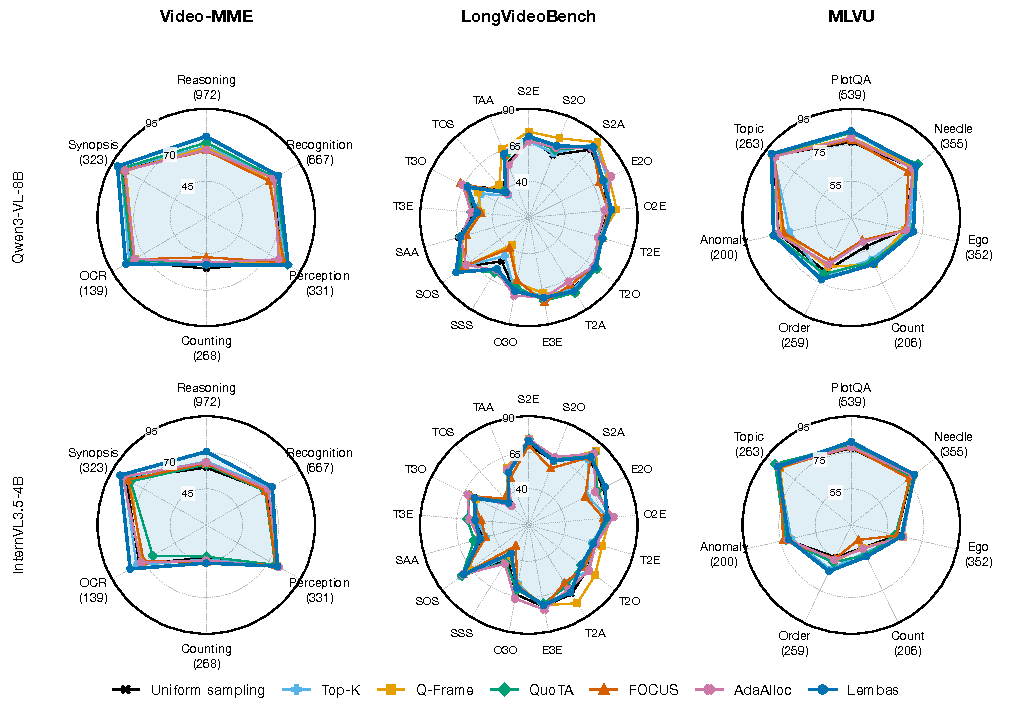
\includegraphics[width=\linewidth]{fig/category_radar.pdf}
  \caption{\textbf{\name achieves the highest accuracy in most question categories of Video-MME and MLVU.} Accuracy (\%) per question category; columns are benchmarks and rows are VLMs, and each benchmark shares one radial scale across both VLMs. Numbers in parentheses are question counts. Video-MME groups its 12 task types into six as in Q-Frame~\cite{zhang2025qframe}; LongVideoBench uses its 17 question categories.}
  \label{fig:supp-radar}
\end{figure*}

\begin{figure*}[t]
  \centering
  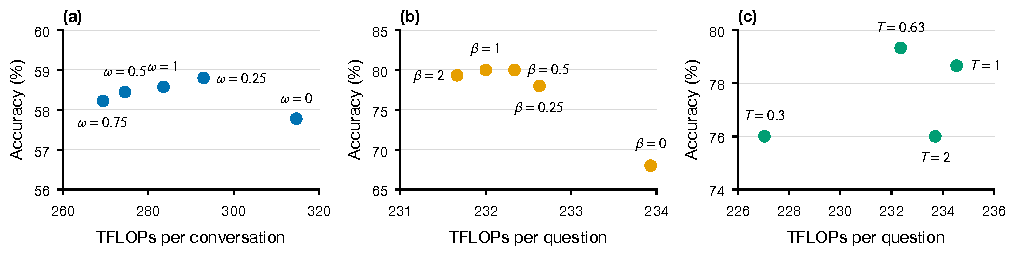
\includegraphics[width=\linewidth]{fig/sens_panels.pdf}
  \caption{\textbf{\name is robust to its manually chosen settings.} Accuracy against compute when varying (a) the attention weight $\omega$ on MT-Video-Bench, (b) the subtitle weight $\beta$ on Video-MME, and (c) the relevance temperature $T$ on Video-MME, with all other settings fixed. The sweeps use subsets of 200 conversations (a), 150 questions (b), and 300 questions (c).}
  \label{fig:supp-sens}
\end{figure*}

\subsection{Per-Category Accuracy}
\label{sec:supp-category}

\Cref{fig:supp-radar} breaks down the accuracy in Tab.~1 of the main paper by question category. On Video-MME, \name achieves the highest accuracy in five of the six task groups with both VLMs, and its largest gains are on reasoning questions (4.2 and 6.8 points over the best baseline with Qwen3-VL-8B and InternVL3.5-4B, respectively). On MLVU, \name achieves the highest accuracy in six of the seven tasks with Qwen3-VL-8B (one tied with Q-Frame) and in four with InternVL3.5-4B. The gains of \name thus hold across question categories and do not come from a single one.

\subsection{Solver Efficiency}
\label{sec:supp-solver}

We compare iterative water-filling with three off-the-shelf solvers. Gurobi~\cite{gurobi} and SCIP~\cite{scip} are integer solvers that solve the discrete allocation problem to optimality, and CVXPY~\cite{cvxpy} with the Clarabel solver~\cite{clarabel} solves the same continuous relaxation as iterative water-filling. We use synthetic videos of 30 to 3,600 candidate frames with 64-dimensional frame embeddings and a time limit of 10 minutes. As shown in \cref{tab:supp-solver}, iterative water-filling is 1.3--7$\times$ faster than CVXPY and 4--23$\times$ faster than Gurobi, while SCIP does not finish within the time limit beyond 420 frames. The objective of iterative water-filling stays within 0.04\% of the integer optimum. With the 1,152-dimensional embeddings of SigLIP~2, Gurobi takes 12.7 seconds for 3,600 frames, whereas iterative water-filling takes 0.24 seconds.

\subsection{Sensitivity Analysis}
\label{sec:supp-sens}

\name has three manually chosen settings, namely the attention weight $\omega$, the subtitle weight $\beta$, and the relevance temperature $T$. \Cref{fig:supp-sens} varies each setting while keeping the other settings fixed. For the attention weight (\cref{fig:supp-sens}a), every $\omega>0$ improves over retrieval relevance alone ($\omega=0$) in both accuracy and compute, and the accuracies for $\omega>0$ differ by less than one point. For the subtitle weight (\cref{fig:supp-sens}b), the accuracies for $\beta>0$ stay within 2 points of each other. With $\beta=0$, no subtitle receives tokens and the prompt contains no subtitles at all, which reduces accuracy by 12 points. This setting differs from the ``w/o text allocation'' row of Tab.~2 of the main paper, which still shows the subtitles aligned with the selected frames, as for the baselines. For the relevance temperature (\cref{fig:supp-sens}c), accuracy is highest at the default $T=0.63$, remains within one point at $T=1$, and drops by about 3 points when $T$ is much smaller or larger. \name is, therefore, robust to $\omega$ and $\beta$ over a wide range, and to $T$ near its default value.
